\begin{center}
	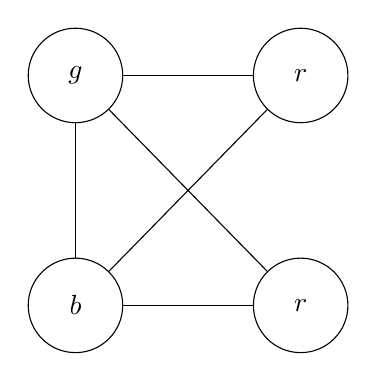
\begin{tikzpicture}[scale=0.2]
		\tikzstyle{every node}+=[inner sep=0pt]
		\draw [black] (9.5,-6.3) circle (3);
		\draw ((9.5,-6.3) node {$g$};
		\draw [black] (23.8,-6.3) circle (3);
		\draw (23.8,-6.3) node {$r$};
		\draw [black] (9.5,-20.9) circle (3);
		\draw (9.5,-20.9) node {$b$};
		\draw [black] (23.8,-20.9) circle (3);
		\draw (23.8,-20.9) node {$r$};
		\draw [black] (11.6,-8.44) -- (21.7,-18.76);
		\draw [black] (9.5,-9.3) -- (9.5,-17.9);
		\draw [black] (12.5,-20.9) -- (20.8,-20.9);
		\draw [black] (12.5,-6.3) -- (20.8,-6.3);
		\draw [black] (11.6,-18.76) -- (21.7,-8.44);
	\end{tikzpicture}
\end{center}